\chapter{\textbf{Metodología}}
\label{chapter:metodologia}

\subsection*{Diagramas de bloques}
\phantomsection
\addcontentsline{toc}{section}{Diagramas de bloques}
\vspace{5mm}

\begin{itemize}
    \item \textbf{Diagrama de bloques del sistema}: es imprescindible presentar en el informe un diagrama de bloques que explique la arquitectura del sistema implementado.
    \item \textbf{Diagrama de bloques de la imagen}: en casos donde el diagrama de bloques del sistema deba abstraerse demasiado para la comprensión del proyecto, será necesario realizar un diagrama de bloques particular para la imagen donde se muestre cómo se procesa.
\end{itemize}

La Figura \ref{fig:diagrama} muestra un resumen de los módulos de software y pueden ayudarle a esbozar sistema (y diagramas).

\begin{figure}[H]
    \centering
    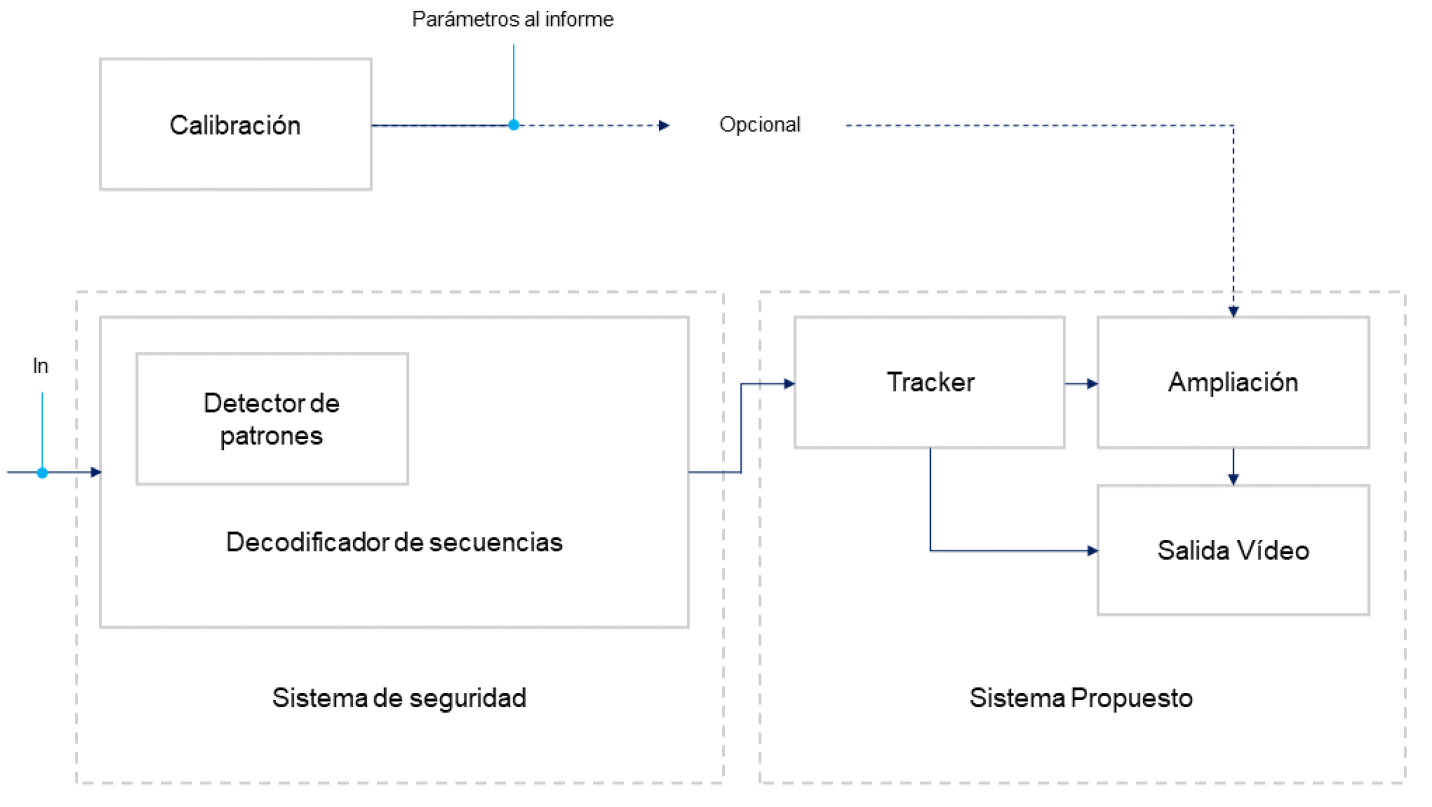
\includegraphics[width=0.85\textwidth]{Lab_Project/template/figures/diagrama.png}
    \caption{Sistema con módulos mínimos. En el módulo calibración se deberá implementar el método de calibración y el de corrección de la distorsión.}
    \label{fig:diagrama}
\end{figure}